\section{Results}

% \subsection{Spatial Properties}

% \begin{enumerate}
% \item Window/less
% \item Orientation (North/South facing)
% \item Separation of characteristically different rooms.
% \end{enumerate}

% \subsubsection{Methdology}

% \subsubsection{Results}
% \begin{figure*}[ht!]
% \centering
% 	\begin{subfigure}{0.48\textwidth}
%                 \centering
% 		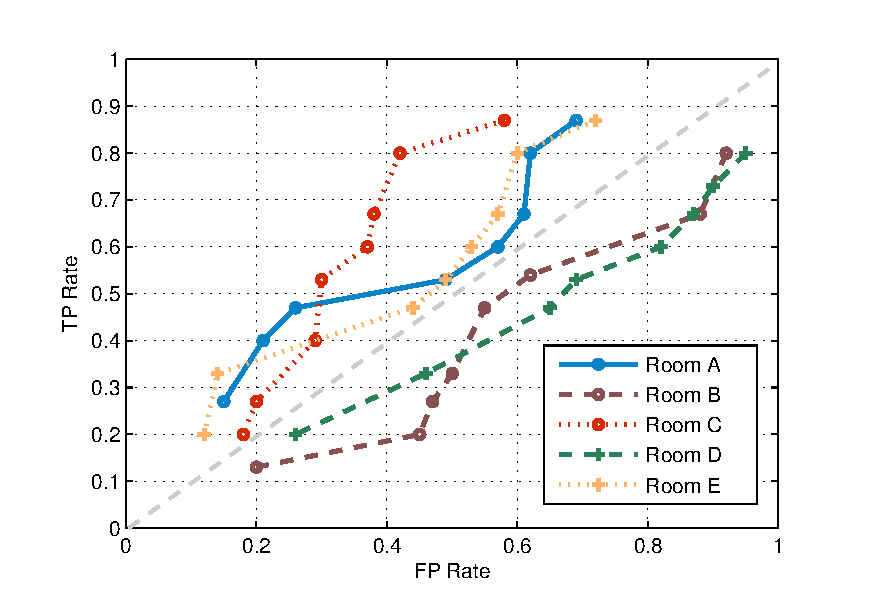
\includegraphics[width=\textwidth]{./fig/ROC_bsln.eps}
%                 \caption{Correlating the raw signals.}
% 	\end{subfigure}
% 	\begin{subfigure}{0.48\textwidth}
%                 \centering
% 		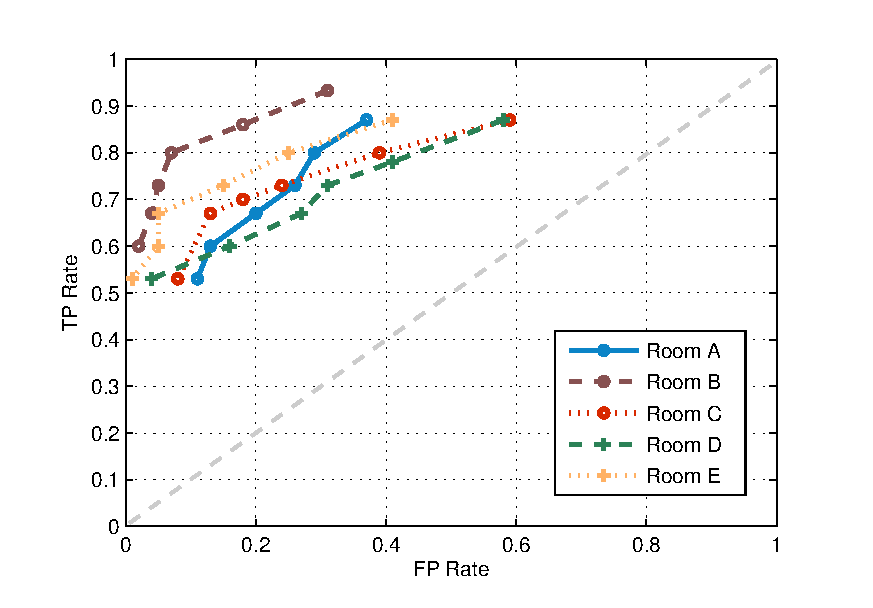
\includegraphics[width=\textwidth]{./fig/ROC_new.eps}
%                 \caption{Correlating the re-aggregated IMFs in the ``medium'' frequency band.}
%                 \label{fig:rocA}
% 	\end{subfigure}
% \caption{The ROC curves depict the sensitivity of the raw signal and mid-frequency IMFs to the threshold value. We choose the 0.2 FPR point as the boundary threshold for each room. }
% \label{fig:roc}
% \end{figure*}

% \section{Experimental Results}
% We conduct two sets of experiments. First, we quantify the sensitivity of our method for different threshold values 
% and examine the effect of different time spans on the threshold. We then cluster the traces based on our threshold analysis 
% and compare it with a baseline approach using multidimensional scaling and k-means.
% % as well as with an approach combining multidimensional scaling and k-meas. 
% % Last, we validate the usefulness of the proposed method in a case study.

% \subsection{Experimental Setup}
% \begin{figure}[h!]
% \centering
%   \includegraphics[width=0.45\textwidth]{./figs/SDH3_crop}
% \caption{We collect data from 15 sensors in 5 rooms sitting on 4 different floors. This is a map of a section of the 3rd floor
% in Sutardja Dai Hall.}
% \label{fig:sdh}
% \end{figure}

% We perform an empirical study on sensor data collected from 15 sensors across 5 rooms on 4 different floors of a large building, as detailed in Table~\ref{table:roomspec}. 
% Each room has three sensors: a temperature sensor, a $CO_{2}$ sensor,  and a humidity sensor. 
% The data from these is reported to an sMAP~\cite{smap} archiver. The data set used comes from a deployment~\cite{Jay} lasting 
% over 6 months on several floors in Sutardja Dai Hall (SDH) at UC Berkeley, where one sensor box -- which contains a thermometer, a humidity sensor and a $CO_{2}$ sensor -- is placed in each room. The box reports data over 6LowPAN~\cite{6lowpan} to a sMAP archiver every 15 seconds. 
%  % The other is a long-term deployment comprised of thousands of sensors that are part of the Building Management System (BMS).
%  % We choose the portion of the SDH data set where the sensor devices, accessible via BACnet~\cite{BACnet}, report data to the archiver every 
%  %few minutes. 
%  Due to intermittent data loss, we pick a time span without interruption, starting in January until mid-Feburary, 2013, for evaluation.

% \begin{table}[ht!]
% \caption{Room Specs}
% \centering % used for centering table
% \begin{tabular}{c c c c}% centered columns (4 columns)
% \hline %inserts single horizontal lines
% Room\# & Orientation & Floor & Type \\ % inserts table 
% %heading
% \hline\hline % inserts double horizontal line
% A & West & 2 & Computer Lab \\ % inserting body of the table
% B & South & 4 & Conference Room \\
% C & No Window & 2 & Classroom \\
% D & North & 7 & Conference Room \\
% E & South & 5 & Conference Room \\ % [1ex] adds vertical space
% \hline %inserts single line
% \end{tabular}
% \label{table:roomspec} % is used to refer this table in the text
% \end{table}

% \subsection{Baseline and Metrics}
% % We exploit a simple approach as baseline to compare with our proposed approach: instead of computing the correlation coefficients between re-aggregated IMFs of sensor feeds, we directly use the raw sensor data to do the correlation analysis and generate the two distributions for thresholding approach evaluation similarly to what described previously.

% % As a baseline, we perform correlation analysis on the raw data. We generate two distributions, as previously described, and observe the effects of the choice of threshold on the true/false positive rate.
% As a baseline, after we generate the two distributions described previously, we apply multidimensional scaling (MDS) to the corrcoeff matrix, in order to transform the original high-dimensional relative space to a 3-D space with an absolute origin, and run the k-means clustering algorithm.
% We choose the true-positive rate (TPR, also known as recall rate) and false-positive rate (FPR) as metrics to evaluate the performance of our method versus the naive approach, which correlates the raw traces. A true-positive (TP) is when a sensor pair in a room is classified as being co-located 
% while a false-positive (FP) is when a sensor that is not in room is classified as being so.
% %is that a sensor not in room A is clustered as in room A.

% \begin{figure}[h!]
% \centering
% 	\includegraphics[width=0.45\textwidth]{./figs/Inter_intra_relationships}
% \caption{Two populations are examined for our threshold analysis.  A solid line connects sensors in the same room while a dotted line connects
%  to a pairs in different rooms.}
% \label{fig:group}
% \end{figure}

% \begin{figure}[h!]
% \centering
% 	% \begin{subfigure}{0.22\textwidth}
%  %                \centering
% 	% 	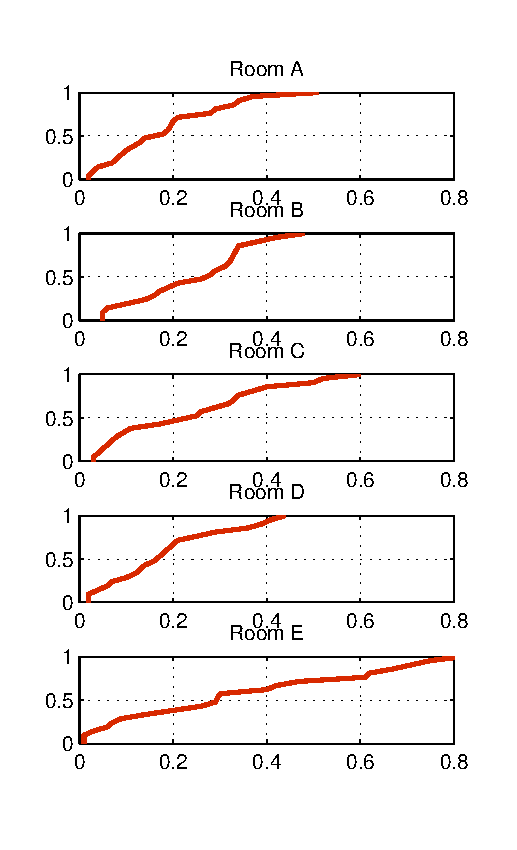
\includegraphics[width=\textwidth]{./fig/cdf_intra.eps}
%  %                \caption{Pairs in the same room}
%  %                \label{fig:cdf_intra}
% 	% \end{subfigure}
% 	% \begin{subfigure}{0.22\textwidth}
%  %                \centering
% 	% 	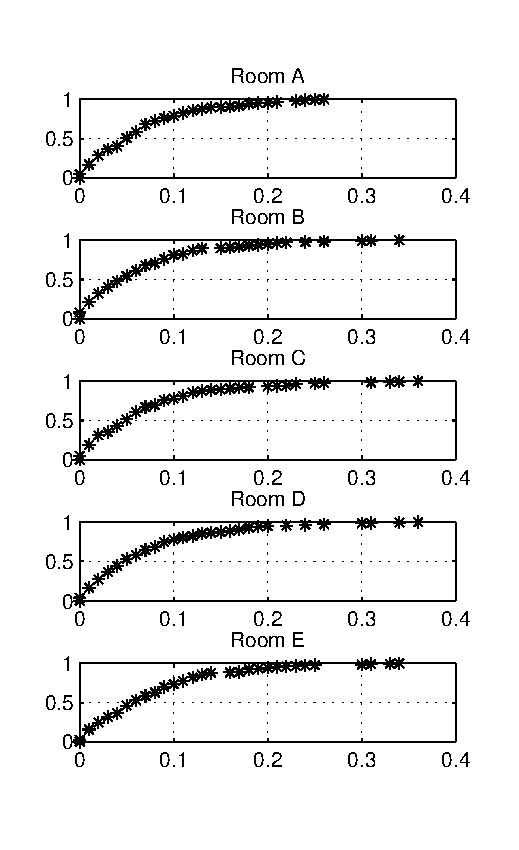
\includegraphics[width=\textwidth]{./fig/cdf_inter.eps}
%  %                \caption{Pairs in different rooms}
%  %                \label{fig:cdf_inter}
% 	% \end{subfigure}
% 	\includegraphics[width=0.45\textwidth]{./figs/corrcoeff_cdf_in_out}
% \caption{CDF of correlation coefficients between IMFs of sensor feeds: the dotted lines point to some threshold which divides
%  the distribution and produces a TPR and FPR.
% % (a) On average, the recall rate of clustering sensors inside one room is (0.62, 0.86). (b) The 80\% corrcoeffs between sensor feeds in rooms falls into (0.1, 0.12).
% }
% \label{fig:cdf}
% \end{figure}

% \subsection{Characterizing the Boundary}
% To corroborate our boundary-existence hypothesis, we first need to characterize the boundary between sensors in different rooms. 
% We compute the pairwise correlation coefficients (corrcoeffs) between sensor traces in both of populations depicted in Figure~\ref{fig:group}, 
% over different time spans -- ranging from one day to one month.
%  % or specifically, 1-3-5-7-14-21-28 days. 
%  % We then generate distributions of the corrcoeffs for each set. 
% After generating points over different time 
% spans for each room, we accumulate the corrcoeffs to obtain distributions as shown in Figure~\ref{fig:cdf}, for each of the five rooms. 

% The dashed vertical lines in Figure~\ref{fig:cdf} 
% represent an arbitrary threshold that partitions the distribution into two sets.  Pairs of sensors to the right of the line
% are classified as being in the same room.  Pairs of sensors to the left are classified as being in different rooms.
% The CDFs on the left column show the distribution of corrcoeffs for pairs known to be in the same room and the CDFs on the right
% show the distribution of corrcoeffs in different rooms.
% Note in the figure, we set the threshold to the same value to both the left and right side, in order to observe the effect of the true/false positive
% rates.
% % point to a same corrcoeff value on the x-axes cutting the two distributions: in the left subfigure, sensor pairs with corrceff to the right of the line are clustered as in the same room, producing a TPR, while in the right subfigure a pair with a corrcoeff to the right of the line is clusted as in the same room, producing a FPR. 
% By adjusting the threshold, we get different TPRs/FPRs parameterized by the threshold. Figure~\ref{fig:roc} captures the range tradeoff in a corresponding ROC curve.
% % pick different corrcoeff values on the CDF curves 
% % from Figure~\ref{fig:cdf_intra} that produce different TPRs and apply the same value as boundary parameters to the corresponding graph
% %  in Figure~\ref{fig:cdf_inter} to obtain the FP rates. 


% Figure~\ref{fig:roc} illustrates the TPR/FPR sensitivity to different threshold values for our method and the naive approach. A good cluster achieves a high TPR and a low FPR. 
% As we vary the threshold, we see that our approach 
% achieves a TPR between 52\%--93\% and a FPR between 5\%--59\%.  %The baseline, mostly remains along the diagonal, meaning it is practically random. 
% We can see that the average TPR for the ROC graph on the right is higher than the 
% ROC graph on the left.  Moreover, the corresponding average FPR is lower on the right than on the left.
%  %From the ROC curves, statistically, our approach is able to accomplish much higher TPRs while maintaining lower FPRs compared to the baseline. 
% In general, as the TPR rises, the FPR also goes up -- \emph{a tradeoff exists between maximizing TPR and maintaining a lower FPR}.
%  % In Figure~\ref{fig:cdf}, a threshold parameter of lower probability from the left will have more sensors 
%  % being correctly classified as being 
%  % in the same room (equivalent to a higher TPR) while letting more sensors in different rooms on the right be incorrectly clustered as in the same room 
%  % (equivalent to a higher FPR).  Consequently, we need to find an optimal threshold parameter to balance the TPR and FPR.

%  The ``boundary'' is represented as the corrcoeff that produces a ``good" TPR with an ``acceptable" FPR.  In Figure~\ref{fig:rocA}, 
%   we choose 0.2 FPR as the boundary threshold.  This point represents the largest difference between TPR and FPR -- an acceptable tradeoff point. 
% Looking at Figure~\ref{fig:cdf}, the 0.2 FPR corresponds roughly to the 80th-percentile correlation coefficient, on the ``inter''
% set (the set of CDFs on the right).
% % The dots in 
%   % Figure~\ref{fig:cdf_intra} present the corresponding approximate recall rates (1-y value) of sensors in each room using 
%   % the same threshold parameters from the counterpart on the right (the 80 percent corrcoeff). 
%   The recall rate for each room -- using a 80th-percentile corrcoeff threshold value -- ranges between 62\%-86\% and the 
%   threshold value falls into a narrow interval between 0.1 to 0.12. This shows that \emph{we are able to choose a uniform value 
%   for all the rooms regardless of the sensor type.}

% \subsection{Convergence over Time}
% \begin{figure}[h!]
% \centering
% 	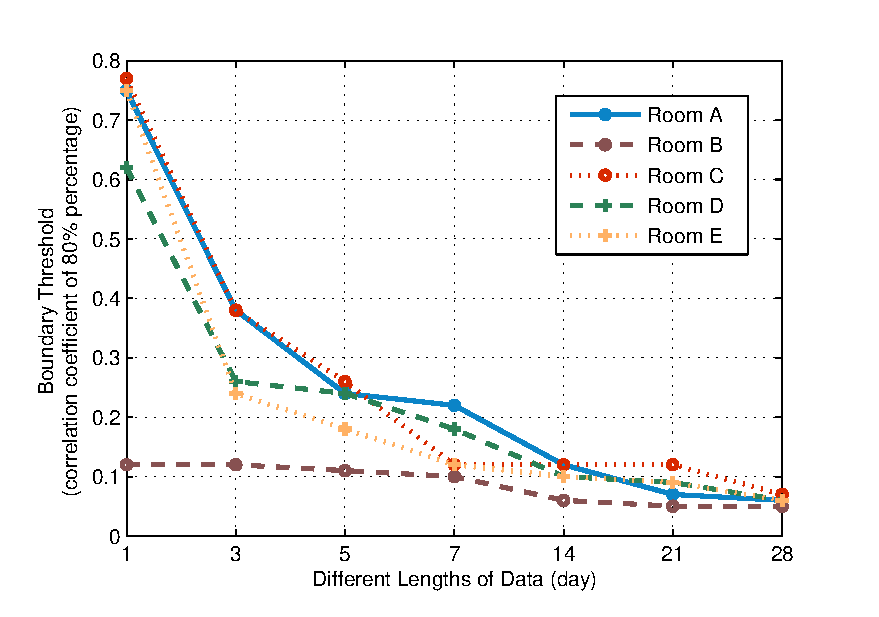
\includegraphics[width=0.48\textwidth]{./figs/lengtheffect.eps}
% \caption{The threshold values all converge to a similar value and we can derive the optimal value with as minimal as 14 days data.}
% \label{fig:leneff}
% \end{figure}

% % With the above decision on choosing the 80\% percentage corrcoeff as a threshold parameter, we also examine how the discriminator value responses to different time spans and whether the value converges as this is critical to automate the process of threshold parameter choice. 
% Using the threshold the roughly 80th-percentile corrcoeff corresponds to in the distribution, we examine how it affects the classification rate across traces
% that span different lengths of time.  Convergence and consistency across different time spans is critical to automate the parameter selection
% process.
% % To test the effect of data length on the threshold value, we use the corrcoeff distribution of sensor pairs in different rooms 
% % over different time spans and identify the 80\%-percentile corrcoeff values. 
% Observe how the  threshold values differ quite significantly in Figure~\ref{fig:leneff}.  However, 
% the threshold values 
% gradually converge, as the length of training data increases from one day to one month.  The values derived after 14 days of data
% are approximately the same as the final convergence value (around 0.07).  In other words, we can determine a threshold from two weeks of data.
% %  and cluster
% % after 14 days or longer time period, the discriminator values for all the rooms converge to almost the same point.
% \subsection{Clustering Results}
% We cluster the sensor traces over the entire one-month period, and use the roughly 80th percentile corrceff (0.07) as the boundary threshold. 
% % Note, a sensor can have corrcoeffs greater than the threshold with sensors in more than one room. When this occurs, 
% A sensor is classified into the cluster with the largest corrcoeff. The clustering result is shown in Table~\ref{tab:cluster}.  A ``1" means the sensor is classified as inside the corresponding room. 
% In general, after obtaining the sensor clusters, we don't know which room each cluster corresponds to without further information such as the metadata of sensors. The labels ``A-E" in Table~\ref{tab:cluster} are used to indicate the ground truth of where each sensor is physically placed since we have such information. Overall, the classification accuracy 
% % (defined as the number of correctly clustered sensors compared to total 
% % attempted clustering) 
% is 93.3\%.  We do not cluster on the corrcoeffs obtained among raw signals because the 80\%-percentile corrcoeff values do not converge across rooms.
% The reason that we are able to get such a high accuracy, which is seemingly different from the statistics in Figure~\ref{fig:cdf} and Figure~\ref{fig:roc}, is because the statistics in the two figures are generated out of the corrcoeffs accumulated over different time spans (the same intervals in Figure~\ref{fig:leneff}) while the clustering here is performed on the corrcoeffs from the entire one-month period. 
% % vary a lot and it doesn't make much sense to use different threshold for each room individually.

% \begin{table}[h!]\footnotesize
%  \begin{center}
% 	\begin{tabular}{ r|c|c|c|c|c|c }
% 	\multicolumn{1}{r}{}
% 	 &  \multicolumn{1}{c}{$A$}
% 	 & \multicolumn{1}{c}{$B$}
% 	 & \multicolumn{1}{c}{$C$}
% 	 & \multicolumn{1}{c}{$D$}
% 	  & \multicolumn{1}{c}{$E$} \\
% 	\cline{2-6} 
% 	$SensorA_{1}$ & 1 & 0 & 0 & 0 & 0 & \checkmark\\
% 	\cline{2-6}
% 	$A_{2}$ & 1 & 0 & 0 & 0 & 0 & \checkmark\\
% 	\cline{2-6}
% 	$A_{3}$ & 1 & 0 & 0 & 0 & 0 & \checkmark\\
% 	\cline{2-6}
% 	$B_{1}$ & 0 & 1 & 0 & 0 & 0 & \checkmark\\
% 	\cline{2-6}
% 	$B_{2}$ & 0 & 1 & 0 & 0 & 0 & \checkmark\\
% 	\cline{2-6}
% 	$B_{3}$ & 0 & 1 & 0 & 0 & 0 & \checkmark\\
% 	\cline{2-6}
% 	$C_{1}$ & 0 & 0 & 1 & 0 & 0 & \checkmark\\
% 	\cline{2-6}
% 	$C_{2}$ & 0 & 0 & 1 & 0 & 0 & \checkmark\\
% 	\cline{2-6}
% 	$C_{3}$ & 0 & 0 & 1 & 0 & 0 & \checkmark\\
% 	\cline{2-6}
% 	$D_{1}$ & 0 & 0 & 0 & 1 & 0 & \checkmark\\
% 	\cline{2-6}
% 	$D_{2}$ & 0 & 0 & 0 & 1 & 0 & \checkmark\\
% 	\cline{2-6}
% 	$D_{3}$ & 0 & 0 & 1 & 0 & 0 & $\times$\\
% 	\cline{2-6}
% 	$E_{1}$ & 0 & 0 & 0 & 0 & 1 & \checkmark\\
% 	\cline{2-6}
% 	$E_{2}$ & 0 & 0 & 0 & 0 & 1 & \checkmark\\
% 	\cline{2-6}
% 	$E_{3}$ & 0 & 0 & 0 & 0 & 1 & \checkmark\\
% 	\cline{2-6}
% 	\end{tabular}
%  \end{center}
%  \caption{Clustering result using the thresholding method: a ``1" means the sensor is classified as inside the room. We get the ``\checkmark" and ``$\times$" by comparing the clustering results with ground truth.}
%  \label{tab:cluster}
% \end{table}

% \begin{figure*}[ht!]
% \centering
% 	\begin{subfigure}{0.48\textwidth}
%                 \centering
% 		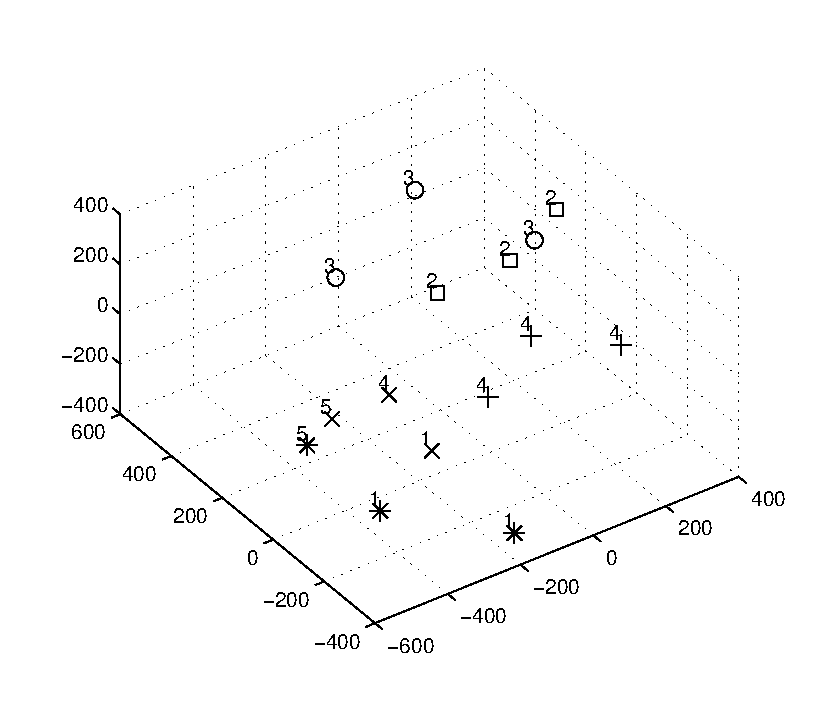
\includegraphics[width=\textwidth]{./figs/res_emd.eps}
%                 \caption{Clustering on corrcoeffs from our method.}
%                 \label{fig:res_emd}
% 	\end{subfigure}
% 	\begin{subfigure}{0.48\textwidth}
%                 \centering
% 		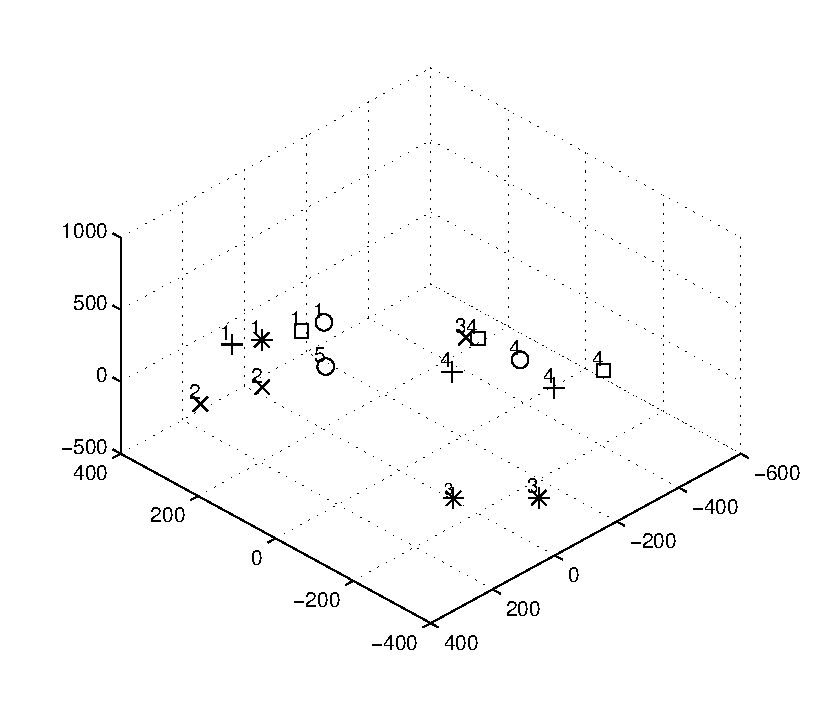
\includegraphics[width=\textwidth]{./figs/res_bsln.eps}
%                 \caption{Clustering on corrcoeffs from the naive approach.}
%                 \label{fig:res_bsln}
% 	\end{subfigure}
% \caption{Clustering with k-means on the corrcoeff matrix after applying multidimensional scaling (MDS): The EMD-based set achieves an accuracy of 80\% while the results with raw-trace is only 53.3\% classification accuracy.}
% \label{fig:mds}
% \end{figure*}

% To compare with our threshold-based method, we also cluster using a baseline approach. The pairwise corrcoeff for sensors in different rooms can be interpreted as a ``distance" between them.
% A larger coefficient indicates a closer ``distance", and vice versa.  However, since the distances between pairs is relative, we use
% multidimensional scaling~\cite{MDS} to find a common basis in three dimensions, re-map the relative distance metric (feature vector) into 
% this three-dimensional grid and use k-means to classify the traces. % assuming the value of k is known a priori, which is the number of rooms.
% We set k to equal the number of rooms, since the goal of the approach is to verify spatial placement at room-level granularity.  Generally, 
% we believe that k should equal the number of rooms you wish to classify the sensors into.
% % Such distances between points corresponds to the dissimilarities between 
% % a pair in the original high-dimensional space which is inviable to visualize. 
% %Therefore, we use Multidimensional Scaling \cite{MDS} to decrease the dimension of corrcoeff matrix to a 3-D space and use k-means to do the clustering. 
% The clustering results are shown in Figure~\ref{fig:mds}.  Ground truth is shown through different markers (x, o, +, star, box). Each marker stands for one room. 
% The cluster each sensor assigned to is denoted with a number. The classification accuracy of the baseline approach on corrcoeffs matrix of re-aggregated IMFs is 80\%. 
% For raw traces, the baseline approach achieves an accuracy of only 53.3\%.





\subsection{Categorical Properties}

\begin{enumerate}
\item Soda Hall data (ART, OAT, VAV, RVAV)
\item Todai data
\item KETI data
\end{enumerate}

\subsection{Methodology}

\subsection{Results}


%\begin{figure*}[htb!]
%\begin{center}
%\includegraphics[width=18cm]{../figs/channel_comp}
%\caption{RSSI measurements for specific channels over time. The values are averaged over a minute. Most sensor networks are set to channel 26 to minimize chance of interference, but in this case, channel 15 is significantly better}
%\label{channelcomp}
%\end{center}
%\end{figure*}

